\documentclass[11pt]{article}
\usepackage{mathblatt}
% gesetzt von werkzeuge/setzer.py (Sorte selbst) aus dem Lernweg FS9
% und den Bankzeilen; Muster bau/proben/2026-10-09/hypotenuse-muster.
\usepackage{enumitem}
\usepackage{adjustbox,varwidth}
\newgeometry{a4paper,margin=18mm,top=15mm,bottom=20mm,footskip=9mm}
\pagestyle{fancy}\fancyhf{}\renewcommand{\headrulewidth}{0pt}
\fancyfoot[L]{\footnotesize\color{mbgrau}FS9 \textperiodcentered{} Brüche vergleichen und ordnen}
\fancyfoot[R]{\footnotesize\color{mbgrau}\thepage}
\setlength{\parskip}{3pt}
\renewcommand{\kreuz}[1]{\mbox{$\square$\ #1}\quad}
\newcommand{\kreuzl}[1]{\par\hangindent1.4em\hangafter1\noindent$\square$\ #1}
\newcommand{\aufg}[3]{\par\noindent\makebox[0pt][r]{#3}\begin{minipage}[t]{\linewidth}#1\end{minipage}\par}
\newcommand{\aufgg}[4]{\par\noindent\makebox[0pt][r]{#4}\begin{minipage}[t]{0.6\linewidth}\vspace{0pt}#1\end{minipage}\hfill
  \begin{minipage}[t]{0.37\linewidth}\vspace{0pt}\centering #2\end{minipage}\par}
\newcommand{\nr}[1]{\makebox[7mm][l]{\textbf{#1}}}
\newcommand{\lsg}[3]{\par\noindent\begin{minipage}[t]{9mm}\textbf{#1}\end{minipage}%
  \begin{minipage}[t]{52mm}\raggedright\bfseries\boldmath #2\end{minipage}\hspace{3mm}%
  \begin{minipage}[t]{\dimexpr\linewidth-64mm\relax}\raggedright\small #3\end{minipage}\par\vspace{4pt}}
\newlength{\kr}
\makeatletter
\newcommand{\karomerk}[2]{\protected@write\@auxout{}{\string\karoseite{#1}{#2}{\thepage}}}
\newcommand{\karoseite}[3]{\expandafter\xdef\csname karo@#1@#2\endcsname{#3}}
\newcommand{\karohinweis}[3]{\karomerk{h}{#1}\ifcsname karo@k@#1\endcsname
  \ifnum\csname karo@k@#1\endcsname=0\csname karo@h@#1\endcsname\relax#2\else#3\fi
  \else#3\fi}
\makeatother
\begin{document}

\noindent{\LARGE\bfseries Brüche vergleichen und ordnen}\par\smallskip
\noindent{\small\color{mbgrau}Selbstlernheft Klasse 6 \textperiodcentered{} mit Lösungsheft \textperiodcentered{} Kennung FS9}\par\medskip
\noindent\textbf{So nutzt du das Heft:} Lies im Abschnitt das Beispiel. Rechne dann die Aufgaben der Reihe nach und vergleiche jede sofort mit dem Lösungsheft. Kreuze „kann ich“ an, wenn du die letzte Aufgabe (\emph{Ziel}) allein schaffst.\par
\noindent Mehr Aufgaben zu einem Abschnitt: Kennung deinem Nachhilfelehrer schicken (z.\,B. „FS9 mehr B“).\par\medskip
{\arrayrulecolor{mbgrau}\renewcommand{\arraystretch}{1.3}
\noindent\begin{tabular}{|>{\bfseries}p{10mm}|p{112mm}|>{\raggedleft\arraybackslash}p{10mm}|>{\centering\arraybackslash}p{14mm}|}\hline
\rowcolor{black!8} & \textbf{Abschnitt} & \textbf{Seite} & \textbf{kann ich}\\\hline
A & Gleicher Nenner oder gleicher Zähler & \pageref{s:A} & $\square$\\\hline
B & Gleichnamig machen, dann vergleichen & \pageref{s:B} & $\square$\\\hline
C & Am Zahlenstrahl: ablesen, eintragen, ordnen & \pageref{s:C} & $\square$\\\hline
D & Einen Bruch dazwischen finden & \pageref{s:D} & $\square$\\\hline
T & Probetest & \pageref{s:T} & $\square$\\\hline
\end{tabular}}\par\bigskip

\begin{tcolorbox}[colback=mbkasten,colframe=mbgrau,boxrule=0.5pt,arc=1mm,left=3mm,right=3mm,top=2mm,bottom=2mm,title={\bfseries Formel auf einen Blick},coltitle=black,colbacktitle=black!10]
{\Large $<$ \ heißt „kleiner als“ \qquad $>$ \ heißt „größer als“ \qquad erweitern: $\dfrac{Z}{N} = \dfrac{Z \cdot k}{N \cdot k}$}\par\medskip
In Worten: Die Spitze von $<$ und $>$ zeigt immer auf die kleinere Zahl. Erweitern ändert die Größe eines Bruchs nicht.\par\medskip
\end{tcolorbox}
\medskip\noindent\textbf{Typische Fehler – so nicht}\par\smallskip
\noindent\nr{$\times$}Zähler und Nenner einzeln verglichen: $3 < 4$ und $5 < 7$ – trotzdem ist $\dfrac{3}{5} > \dfrac{4}{7}$, denn $\dfrac{21}{35} > \dfrac{20}{35}$.\par
\noindent\nr{$\times$}„Bei beiden fehlt nur ein Stück, also sind sie gleich groß“: $\dfrac{2}{3} < \dfrac{4}{5}$, denn $\dfrac{10}{15} < \dfrac{12}{15}$.\par
\clearpage\label{s:A}\noindent\colorbox{black!12}{\makebox[10mm]{\Large\bfseries\strut A}}\hspace{3mm}{\Large\bfseries Gleicher Nenner oder gleicher Zähler}\par\smallskip
\noindent Bei \textbf{gleichem Nenner} sind alle Teile gleich groß: Der Bruch mit dem größeren Zähler ist größer. Bei \textbf{gleichem Zähler} hast du gleich viele Teile: Je größer der Nenner, desto kleiner jedes Teil – und desto kleiner der Bruch.\par\medskip
\noindent\textbf{Formel}\par\nopagebreak\noindent\hspace*{4mm}\begin{minipage}{\dimexpr\linewidth-4mm\relax}$\dfrac{3}{7} < \dfrac{5}{7}$ \ (gleicher Nenner) \qquad $\dfrac{2}{5} > \dfrac{2}{9}$ \ (gleicher Zähler)\end{minipage}\par\medskip
\noindent\textbf{Beispiel}\quad Vergleiche $\dfrac{3}{8}$ mit $\dfrac{5}{8}$ und $\dfrac{3}{8}$ mit $\dfrac{3}{5}$.\par\smallskip
\noindent\begin{minipage}[t]{0.6\linewidth}\vspace{0pt}\par\noindent\hangindent6mm\hangafter1\makebox[6mm][l]{\textbf{1}}$\dfrac{3}{8}$ und $\dfrac{5}{8}$: gleicher Nenner, beides Achtel. 5 Achtel sind mehr als 3 Achtel: $\dfrac{3}{8} < \dfrac{5}{8}$.\par\smallskip\par\noindent\hangindent6mm\hangafter1\makebox[6mm][l]{\textbf{2}}$\dfrac{3}{8}$ und $\dfrac{3}{5}$: gleicher Zähler. Fünftel sind größer als Achtel – das Ganze ist in weniger Teile geteilt.\par\smallskip\par\noindent\hangindent6mm\hangafter1\makebox[6mm][l]{\textbf{3}}3 große Teile sind mehr als 3 kleine: $\dfrac{3}{5} > \dfrac{3}{8}$.\par\smallskip\end{minipage}\hfill
\begin{minipage}[t]{0.37\linewidth}\vspace{0pt}\centering \begin{tikzpicture}[font=\small]\fill[black!25] (0,0.00) rectangle (1.575,0.50);\draw[line width=0.4pt] (0.525,0.00) -- (0.525,0.50);\draw[line width=0.4pt] (1.050,0.00) -- (1.050,0.50);\draw[line width=0.4pt] (1.575,0.00) -- (1.575,0.50);\draw[line width=0.4pt] (2.100,0.00) -- (2.100,0.50);\draw[line width=0.4pt] (2.625,0.00) -- (2.625,0.50);\draw[line width=0.4pt] (3.150,0.00) -- (3.150,0.50);\draw[line width=0.4pt] (3.675,0.00) -- (3.675,0.50);\draw[line width=0.8pt] (0,0.00) rectangle (4.2,0.50);\node[left] at (0,0.25) {$\dfrac{3}{8}$};\fill[black!25] (0,-0.95) rectangle (2.625,-0.45);\draw[line width=0.4pt] (0.525,-0.95) -- (0.525,-0.45);\draw[line width=0.4pt] (1.050,-0.95) -- (1.050,-0.45);\draw[line width=0.4pt] (1.575,-0.95) -- (1.575,-0.45);\draw[line width=0.4pt] (2.100,-0.95) -- (2.100,-0.45);\draw[line width=0.4pt] (2.625,-0.95) -- (2.625,-0.45);\draw[line width=0.4pt] (3.150,-0.95) -- (3.150,-0.45);\draw[line width=0.4pt] (3.675,-0.95) -- (3.675,-0.45);\draw[line width=0.8pt] (0,-0.95) rectangle (4.2,-0.45);\node[left] at (0,-0.70) {$\dfrac{5}{8}$};\fill[black!25] (0,-1.90) rectangle (2.520,-1.40);\draw[line width=0.4pt] (0.840,-1.90) -- (0.840,-1.40);\draw[line width=0.4pt] (1.680,-1.90) -- (1.680,-1.40);\draw[line width=0.4pt] (2.520,-1.90) -- (2.520,-1.40);\draw[line width=0.4pt] (3.360,-1.90) -- (3.360,-1.40);\draw[line width=0.8pt] (0,-1.90) rectangle (4.2,-1.40);\node[left] at (0,-1.65) {$\dfrac{3}{5}$};\end{tikzpicture}\end{minipage}\par\medskip
\noindent\textbf{Aufgaben}\hspace{1em}{\small\color{mbgrau}\karohinweis{A}{Rechne unten im Karo.}{Rechne auf einem extra Blatt.} Vergleiche jede Aufgabe gleich mit dem Lösungsheft.}\par\smallskip
\aufg{\hangindent7mm\hangafter1\nr{1.}Setze $<$ oder $>$ ein. \par\vspace{3pt} a)~$\dfrac{4}{9} \;\square\; \dfrac{7}{9}$ \qquad b)~$\dfrac{11}{12} \;\square\; \dfrac{5}{12}$ \qquad c)~$\dfrac{6}{10} \;\square\; \dfrac{9}{10}$}{}{}
\medskip
\aufg{\hangindent7mm\hangafter1\nr{2.}Setze $<$ oder $>$ ein. \par\vspace{3pt} a)~$\dfrac{2}{3} \;\square\; \dfrac{2}{7}$ \qquad b)~$\dfrac{5}{12} \;\square\; \dfrac{5}{6}$ \qquad c)~$\dfrac{7}{10} \;\square\; \dfrac{7}{8}$}{}{}
\medskip
\aufg{\hangindent7mm\hangafter1\nr{3.}Ordne von klein nach groß: \ $\dfrac{1}{4}$, \ $\dfrac{1}{10}$, \ $\dfrac{1}{3}$, \ $\dfrac{1}{6}$}{}{}
\medskip
\aufg{\hangindent7mm\hangafter1\nr{4.}Jan, Pia und Ole laufen jeder eine gleich lange Runde um den See. Jan hat schon drei Viertel geschafft, Pia drei Fünftel und Ole drei Achtel. Wer ist am weitesten? Wer ist am wenigsten weit?}{}{{\scriptsize\color{mbgrau}Ziel\hspace{2mm}}}
\medskip
\par\vspace{3mm}\setlength{\kr}{\dimexpr\pagegoal-\pagetotal-10mm\relax}%
\ifdim\kr>12mm\karomerk{k}{A}\noindent{\scriptsize\color{mbgrau}Platz zum Rechnen}\par\nointerlineskip\vspace{1mm}\noindent
\begin{tikzpicture}\clip (0,0) rectangle ({\linewidth-0.5mm},\kr);\draw[black!16,line width=0.3pt,step=5mm] (0,0) grid (\linewidth,\kr);\end{tikzpicture}\fi\par
\clearpage\label{s:B}\noindent\colorbox{black!12}{\makebox[10mm]{\Large\bfseries\strut B}}\hspace{3mm}{\Large\bfseries Gleichnamig machen, dann vergleichen}\par\smallskip
\noindent Sind Zähler und Nenner verschieden, kannst du nicht direkt vergleichen. Bring beide Brüche auf denselben Nenner – dann entscheidet der Zähler.\par\medskip
\noindent\textbf{Formel}\par\nopagebreak\noindent\hspace*{4mm}\begin{minipage}{\dimexpr\linewidth-4mm\relax}$\dfrac{2}{3}$ und $\dfrac{3}{5}$: \ $\dfrac{10}{15} > \dfrac{9}{15}$, \ also $\dfrac{2}{3} > \dfrac{3}{5}$ \par\vspace{4pt} {\small Gemeinsamer Nenner: eine Zahl, die in beiden Einmaleins-Reihen steht.}\end{minipage}\par\medskip
\noindent\textbf{Beispiel}\quad Was ist größer: $\dfrac{5}{6}$ oder $\dfrac{7}{8}$?\par\smallskip
\noindent\par\noindent\hangindent6mm\hangafter1\makebox[6mm][l]{\textbf{1}}Gemeinsamer Nenner: 24 steht in der Sechser- und in der Achterreihe.\par\smallskip\par\noindent\hangindent6mm\hangafter1\makebox[6mm][l]{\textbf{2}}Erweitern: $\dfrac{5}{6} = \dfrac{5 \cdot 4}{6 \cdot 4} = \dfrac{20}{24}$ \quad $\dfrac{7}{8} = \dfrac{7 \cdot 3}{8 \cdot 3} = \dfrac{21}{24}$\par\smallskip\par\noindent\hangindent6mm\hangafter1\makebox[6mm][l]{\textbf{3}}Zähler vergleichen: $20 < 21$, also $\dfrac{5}{6} < \dfrac{7}{8}$.\par\smallskip\par\medskip
\noindent\textbf{Aufgaben}\hspace{1em}{\small\color{mbgrau}\karohinweis{B}{Rechne unten im Karo.}{Rechne auf einem extra Blatt.} Vergleiche jede Aufgabe gleich mit dem Lösungsheft.}\par\smallskip
\aufg{\hangindent7mm\hangafter1\nr{1.}Mach gleichnamig und setze $<$ oder $>$ ein. \par\vspace{3pt} a)~$\dfrac{2}{3} \;\square\; \dfrac{5}{6}$ \qquad b)~$\dfrac{3}{4} \;\square\; \dfrac{5}{8}$ \qquad c)~$\dfrac{7}{10} \;\square\; \dfrac{3}{5}$}{}{}
\medskip
\aufg{\hangindent7mm\hangafter1\nr{2.}Mach gleichnamig und setze $<$ oder $>$ ein. \par\vspace{3pt} a)~$\dfrac{2}{3} \;\square\; \dfrac{3}{4}$ \qquad b)~$\dfrac{4}{5} \;\square\; \dfrac{3}{4}$ \qquad c)~$\dfrac{5}{6} \;\square\; \dfrac{7}{9}$}{}{}
\medskip
\aufg{\hangindent7mm\hangafter1\nr{3.}Gleicher Nenner, gleicher Zähler oder keins von beiden? Entscheide erst, dann setze $<$ oder $>$ ein. \par\vspace{3pt} a)~$\dfrac{3}{4} \;\square\; \dfrac{9}{10}$ \qquad b)~$\dfrac{5}{7} \;\square\; \dfrac{5}{9}$ \qquad c)~$\dfrac{2}{5} \;\square\; \dfrac{3}{7}$}{}{}
\medskip
\aufg{\hangindent7mm\hangafter1\nr{4.}Der Ausflug der 6b findet statt, wenn mindestens drei Viertel der Klasse zustimmen. 17 von 24 Kindern stimmen zu. Findet der Ausflug statt? Wenn nicht: Wie viele Stimmen fehlen?}{}{{\scriptsize\color{mbgrau}Ziel\hspace{2mm}}}
\medskip
\par\vspace{3mm}\setlength{\kr}{\dimexpr\pagegoal-\pagetotal-10mm\relax}%
\ifdim\kr>12mm\karomerk{k}{B}\noindent{\scriptsize\color{mbgrau}Platz zum Rechnen}\par\nointerlineskip\vspace{1mm}\noindent
\begin{tikzpicture}\clip (0,0) rectangle ({\linewidth-0.5mm},\kr);\draw[black!16,line width=0.3pt,step=5mm] (0,0) grid (\linewidth,\kr);\end{tikzpicture}\fi\par
\clearpage\label{s:C}\noindent\colorbox{black!12}{\makebox[10mm]{\Large\bfseries\strut C}}\hspace{3mm}{\Large\bfseries Am Zahlenstrahl: ablesen, eintragen, ordnen}\par\smallskip
\noindent Am Zahlenstrahl liegt der kleinere Bruch weiter links. Ist die Strecke von 0 bis 1 in $N$ gleiche Schritte geteilt, ist ein Schritt $\dfrac{1}{N}$. Zum Ordnen sortiere zuerst grob: kleiner als $\dfrac{1}{2}$, zwischen $\dfrac{1}{2}$ und 1, größer als 1.\par\medskip
\noindent\textbf{Formel}\par\nopagebreak\noindent\hspace*{4mm}\begin{minipage}{\dimexpr\linewidth-4mm\relax}kleiner als $\dfrac{1}{2}$: Zähler kleiner als die Hälfte des Nenners, z.\,B. $\dfrac{3}{8}$ (denn $\dfrac{4}{8} = \dfrac{1}{2}$) \par\vspace{4pt} ungerader Nenner: Zähler verdoppeln, z.\,B. $\dfrac{4}{7}$: $2 \cdot 4 = 8 > 7$, also größer als $\dfrac{1}{2}$ \par\vspace{4pt} größer als 1: Zähler größer als Nenner, z.\,B. $\dfrac{7}{6}$\end{minipage}\par\medskip
\noindent\textbf{Beispiel}\quad Lies $A$ ab. Trage $\dfrac{1}{3}$ und $\dfrac{3}{2}$ ein und ordne alle drei.\par\smallskip
\noindent\begin{minipage}[t]{0.6\linewidth}\vspace{0pt}\par\noindent\hangindent6mm\hangafter1\makebox[6mm][l]{\textbf{1}}Von 0 bis 1 sind es 6 gleiche Schritte: Ein Schritt ist $\dfrac{1}{6}$.\par\smallskip\par\noindent\hangindent6mm\hangafter1\makebox[6mm][l]{\textbf{2}}$A$ liegt 5 Schritte hinter 0: $A = \dfrac{5}{6}$.\par\smallskip\par\noindent\hangindent6mm\hangafter1\makebox[6mm][l]{\textbf{3}}$\dfrac{1}{3} = \dfrac{2}{6}$: 2 Schritte. \quad $\dfrac{3}{2} = \dfrac{9}{6}$: 9 Schritte, also hinter der 1.\par\smallskip\par\noindent\hangindent6mm\hangafter1\makebox[6mm][l]{\textbf{4}}Von links nach rechts: $\dfrac{1}{3} < \dfrac{5}{6} < \dfrac{3}{2}$.\par\smallskip\end{minipage}\hfill
\begin{minipage}[t]{0.37\linewidth}\vspace{0pt}\centering \begin{tikzpicture}\draw[->,line width=0.7pt] (0,0) -- (5.75,0);\draw[line width=0.7pt] (0.000,-0.17) -- (0.000,0.17);\node[below] at (0.000,-0.17) {0};\draw[line width=0.4pt] (0.450,-0.1) -- (0.450,0.1);\draw[line width=0.4pt] (0.900,-0.1) -- (0.900,0.1);\draw[line width=0.4pt] (1.350,-0.1) -- (1.350,0.1);\draw[line width=0.4pt] (1.800,-0.1) -- (1.800,0.1);\draw[line width=0.4pt] (2.250,-0.1) -- (2.250,0.1);\draw[line width=0.7pt] (2.700,-0.17) -- (2.700,0.17);\node[below] at (2.700,-0.17) {1};\draw[line width=0.4pt] (3.150,-0.1) -- (3.150,0.1);\draw[line width=0.4pt] (3.600,-0.1) -- (3.600,0.1);\draw[line width=0.4pt] (4.050,-0.1) -- (4.050,0.1);\draw[line width=0.4pt] (4.500,-0.1) -- (4.500,0.1);\draw[line width=0.4pt] (4.950,-0.1) -- (4.950,0.1);\draw[line width=0.7pt] (5.400,-0.17) -- (5.400,0.17);\node[below] at (5.400,-0.17) {2};\fill (2.250,0) circle (1.7pt);\node[above] at (2.250,0.12) {$A$};\fill (0.900,0) circle (1.7pt);\node[above] at (0.900,0.12) {$\dfrac{1}{3}$};\fill (4.050,0) circle (1.7pt);\node[above] at (4.050,0.12) {$\dfrac{3}{2}$};\end{tikzpicture}\end{minipage}\par\medskip
\noindent\textbf{Aufgaben}\hspace{1em}{\small\color{mbgrau}\karohinweis{C}{Rechne unten im Karo.}{Rechne auf einem extra Blatt.} Vergleiche jede Aufgabe gleich mit dem Lösungsheft.}\par\smallskip
\aufgg{\hangindent7mm\hangafter1\nr{1.}Welche Brüche gehören zu $A$, $B$ und $C$?}{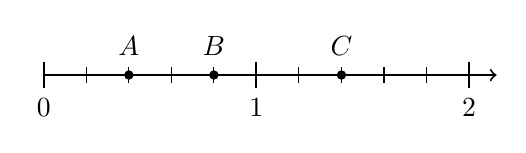
\begin{tikzpicture}\draw[->,line width=0.7pt] (0,0) -- (5.75,0);\draw[line width=0.7pt] (0.000,-0.17) -- (0.000,0.17);\node[below] at (0.000,-0.17) {0};\draw[line width=0.4pt] (0.540,-0.1) -- (0.540,0.1);\draw[line width=0.4pt] (1.080,-0.1) -- (1.080,0.1);\draw[line width=0.4pt] (1.620,-0.1) -- (1.620,0.1);\draw[line width=0.4pt] (2.160,-0.1) -- (2.160,0.1);\draw[line width=0.7pt] (2.700,-0.17) -- (2.700,0.17);\node[below] at (2.700,-0.17) {1};\draw[line width=0.4pt] (3.240,-0.1) -- (3.240,0.1);\draw[line width=0.4pt] (3.780,-0.1) -- (3.780,0.1);\draw[line width=0.4pt] (4.320,-0.1) -- (4.320,0.1);\draw[line width=0.4pt] (4.860,-0.1) -- (4.860,0.1);\draw[line width=0.7pt] (5.400,-0.17) -- (5.400,0.17);\node[below] at (5.400,-0.17) {2};\fill (1.080,0) circle (1.7pt);\node[above] at (1.080,0.12) {$A$};\fill (2.160,0) circle (1.7pt);\node[above] at (2.160,0.12) {$B$};\fill (3.780,0) circle (1.7pt);\node[above] at (3.780,0.12) {$C$};\end{tikzpicture}}{}{}
\medskip
\aufgg{\hangindent7mm\hangafter1\nr{2.}Der Zahlenstrahl ist in Sechstel geteilt. Trage $\dfrac{1}{3}$, $\dfrac{1}{2}$ und $\dfrac{5}{6}$ ein.}{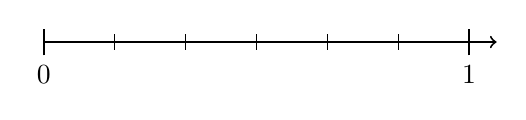
\begin{tikzpicture}\draw[->,line width=0.7pt] (0,0) -- (5.75,0);\draw[line width=0.7pt] (0.000,-0.17) -- (0.000,0.17);\node[below] at (0.000,-0.17) {0};\draw[line width=0.4pt] (0.900,-0.1) -- (0.900,0.1);\draw[line width=0.4pt] (1.800,-0.1) -- (1.800,0.1);\draw[line width=0.4pt] (2.700,-0.1) -- (2.700,0.1);\draw[line width=0.4pt] (3.600,-0.1) -- (3.600,0.1);\draw[line width=0.4pt] (4.500,-0.1) -- (4.500,0.1);\draw[line width=0.7pt] (5.400,-0.17) -- (5.400,0.17);\node[below] at (5.400,-0.17) {1};\end{tikzpicture}}{}{}
\medskip
\aufg{\hangindent7mm\hangafter1\nr{3.}Kleiner als $\dfrac{1}{2}$, zwischen $\dfrac{1}{2}$ und 1 oder größer als 1? Sortiere in drei Gruppen. \par\vspace{3pt} $\dfrac{3}{7}$ \qquad $\dfrac{5}{9}$ \qquad $\dfrac{8}{7}$ \qquad $\dfrac{2}{5}$ \qquad $\dfrac{6}{11}$ \qquad $\dfrac{11}{10}$}{}{}
\medskip
\aufg{\hangindent7mm\hangafter1\nr{4.}Ordne von klein nach groß: \ $\dfrac{5}{6}$, \ $\dfrac{2}{5}$, \ $\dfrac{7}{4}$, \ $\dfrac{3}{8}$}{}{}
\medskip
\aufg{\hangindent7mm\hangafter1\nr{5.}Vier Regentonnen sind verschieden hoch. \par $A$: 50\,cm hoch, 30\,cm Wasser \qquad $B$: 72\,cm hoch, 45\,cm Wasser \par $C$: 80\,cm hoch, 36\,cm Wasser \qquad $D$: 80\,cm hoch, 70\,cm Wasser \par Ordne die Tonnen danach, wie voll sie sind. Welche ist am vollsten?}{}{{\scriptsize\color{mbgrau}Ziel\hspace{2mm}}}
\medskip
\par\vspace{3mm}\setlength{\kr}{\dimexpr\pagegoal-\pagetotal-10mm\relax}%
\ifdim\kr>12mm\karomerk{k}{C}\noindent{\scriptsize\color{mbgrau}Platz zum Rechnen}\par\nointerlineskip\vspace{1mm}\noindent
\begin{tikzpicture}\clip (0,0) rectangle ({\linewidth-0.5mm},\kr);\draw[black!16,line width=0.3pt,step=5mm] (0,0) grid (\linewidth,\kr);\end{tikzpicture}\fi\par
\clearpage\label{s:D}\noindent\colorbox{black!12}{\makebox[10mm]{\Large\bfseries\strut D}}\hspace{3mm}{\Large\bfseries Einen Bruch dazwischen finden}\par\smallskip
\noindent Zwischen zwei Brüchen liegen immer weitere Brüche. Mach beide gleichnamig und wähle einen Zähler dazwischen. Liegt kein Zähler dazwischen, erweitere beide noch einmal, zum Beispiel mit 2.\par\medskip
\noindent\textbf{Formel}\par\nopagebreak\noindent\hspace*{4mm}\begin{minipage}{\dimexpr\linewidth-4mm\relax}$\dfrac{3}{10}$ und $\dfrac{4}{10}$ \ mit 2 erweitert: \ $\dfrac{6}{20} < \dfrac{7}{20} < \dfrac{8}{20}$\end{minipage}\par\medskip
\noindent\textbf{Beispiel}\quad Gib einen Bruch an, der zwischen $\dfrac{3}{5}$ und $\dfrac{2}{3}$ liegt.\par\smallskip
\noindent\par\noindent\hangindent6mm\hangafter1\makebox[6mm][l]{\textbf{1}}Gleichnamig: $\dfrac{3}{5} = \dfrac{9}{15}$, \ $\dfrac{2}{3} = \dfrac{10}{15}$. Zwischen 9 und 10 liegt kein Zähler.\par\smallskip\par\noindent\hangindent6mm\hangafter1\makebox[6mm][l]{\textbf{2}}Beide noch einmal mit 2 erweitern: $\dfrac{18}{30}$ und $\dfrac{20}{30}$.\par\smallskip\par\noindent\hangindent6mm\hangafter1\makebox[6mm][l]{\textbf{3}}Dazwischen liegt $\dfrac{19}{30}$: \ $\dfrac{3}{5} < \dfrac{19}{30} < \dfrac{2}{3}$.\par\smallskip\par\medskip
\noindent\textbf{Aufgaben}\hspace{1em}{\small\color{mbgrau}\karohinweis{D}{Rechne unten im Karo.}{Rechne auf einem extra Blatt.} Vergleiche jede Aufgabe gleich mit dem Lösungsheft.}\par\smallskip
\aufg{\hangindent7mm\hangafter1\nr{1.}Gib zwei Brüche an, die dazwischen liegen. \par\vspace{3pt} a)~$\dfrac{2}{9}$ und $\dfrac{6}{9}$ \qquad b)~$\dfrac{5}{11}$ und $\dfrac{9}{11}$}{}{}
\medskip
\aufg{\hangindent7mm\hangafter1\nr{2.}Gib einen Bruch an, der dazwischen liegt. \par\vspace{3pt} a)~$\dfrac{3}{8}$ und $\dfrac{4}{8}$ \qquad b)~$\dfrac{1}{5}$ und $\dfrac{2}{5}$}{}{}
\medskip
\aufg{\hangindent7mm\hangafter1\nr{3.}Gib einen Bruch an, der dazwischen liegt. \par\vspace{3pt} a)~$\dfrac{1}{3}$ und $\dfrac{3}{4}$ \qquad b)~$\dfrac{2}{5}$ und $\dfrac{1}{2}$}{}{}
\medskip
\aufg{\hangindent7mm\hangafter1\nr{4.}Welcher Bruch liegt zwischen $\dfrac{1}{4}$ und $\dfrac{2}{3}$? Kreuze an.\par\medskip\noindent\hspace*{7mm}\mbox{$\square$\ $\dfrac{1}{5}$}\hspace{10mm}\mbox{$\square$\ $\dfrac{3}{4}$}\hspace{10mm}\mbox{$\square$\ $\dfrac{5}{12}$}\hspace{10mm}\mbox{$\square$\ $\dfrac{7}{10}$}\rule[-3mm]{0pt}{8mm}\par\smallskip }{}{}
\medskip
\aufg{\hangindent7mm\hangafter1\nr{5.}Mia braucht für eine Schleife ein Stück Band. Es soll länger als $\dfrac{1}{5}$\,m und kürzer als $\dfrac{1}{4}$\,m sein. Gib eine passende Länge als Bruch von 1\,m an. Wie viele Zentimeter sind das?}{}{{\scriptsize\color{mbgrau}Ziel\hspace{2mm}}}
\medskip
\par\vspace{3mm}\setlength{\kr}{\dimexpr\pagegoal-\pagetotal-10mm\relax}%
\ifdim\kr>12mm\karomerk{k}{D}\noindent{\scriptsize\color{mbgrau}Platz zum Rechnen}\par\nointerlineskip\vspace{1mm}\noindent
\begin{tikzpicture}\clip (0,0) rectangle ({\linewidth-0.5mm},\kr);\draw[black!16,line width=0.3pt,step=5mm] (0,0) grid (\linewidth,\kr);\end{tikzpicture}\fi\par
\clearpage\label{s:T}\noindent\colorbox{black!12}{\makebox[10mm]{\Large\bfseries\strut T}}\hspace{3mm}{\Large\bfseries Probetest}\par\smallskip
\noindent Gemischt, ohne Beispiel. Etwa 20 Minuten.\par\medskip
\noindent\textbf{Aufgaben}\hspace{1em}{\small\color{mbgrau}\karohinweis{T}{Rechne unten im Karo.}{Rechne auf einem extra Blatt.} Vergleiche jede Aufgabe gleich mit dem Lösungsheft.}\par\smallskip
\aufg{\hangindent7mm\hangafter1\nr{1.}Setze $<$ oder $>$ ein. \par\vspace{3pt} a)~$\dfrac{5}{9} \;\square\; \dfrac{4}{9}$ \qquad b)~$\dfrac{2}{7} \;\square\; \dfrac{2}{5}$ \qquad c)~$\dfrac{3}{4} \;\square\; \dfrac{7}{10}$}{}{}
\medskip
\aufgg{\hangindent7mm\hangafter1\nr{2.}Welche Brüche gehören zu $A$ und $B$? Trage $\dfrac{3}{2}$ ein.}{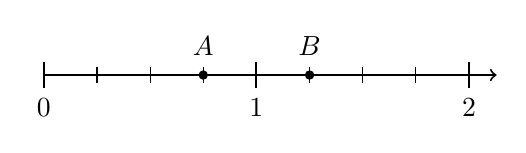
\begin{tikzpicture}\draw[->,line width=0.7pt] (0,0) -- (5.75,0);\draw[line width=0.7pt] (0.000,-0.17) -- (0.000,0.17);\node[below] at (0.000,-0.17) {0};\draw[line width=0.4pt] (0.675,-0.1) -- (0.675,0.1);\draw[line width=0.4pt] (1.350,-0.1) -- (1.350,0.1);\draw[line width=0.4pt] (2.025,-0.1) -- (2.025,0.1);\draw[line width=0.7pt] (2.700,-0.17) -- (2.700,0.17);\node[below] at (2.700,-0.17) {1};\draw[line width=0.4pt] (3.375,-0.1) -- (3.375,0.1);\draw[line width=0.4pt] (4.050,-0.1) -- (4.050,0.1);\draw[line width=0.4pt] (4.725,-0.1) -- (4.725,0.1);\draw[line width=0.7pt] (5.400,-0.17) -- (5.400,0.17);\node[below] at (5.400,-0.17) {2};\fill (2.025,0) circle (1.7pt);\node[above] at (2.025,0.12) {$A$};\fill (3.375,0) circle (1.7pt);\node[above] at (3.375,0.12) {$B$};\end{tikzpicture}}{}{}
\medskip
\aufg{\hangindent7mm\hangafter1\nr{3.}Ordne von klein nach groß: \ $\dfrac{4}{7}$, \ $\dfrac{1}{3}$, \ $\dfrac{5}{4}$, \ $\dfrac{1}{2}$}{}{}
\medskip
\aufg{\hangindent7mm\hangafter1\nr{4.}Gib eine Zahl an, die zwischen $\dfrac{3}{5}$ und $\dfrac{5}{6}$ liegt.}{}{}
\medskip
\aufg{\hangindent7mm\hangafter1\nr{5.}Welche Aussage ist wahr? Kreuze an.\par\medskip\noindent\hspace*{7mm}\mbox{$\square$\ $\dfrac{3}{4} > \dfrac{9}{10}$}\hspace{10mm}\mbox{$\square$\ $\dfrac{5}{8} < \dfrac{1}{2}$}\hspace{10mm}\mbox{$\square$\ $\dfrac{7}{12} > \dfrac{1}{2}$}\hspace{10mm}\mbox{$\square$\ $\dfrac{2}{9} > \dfrac{2}{7}$}\rule[-3mm]{0pt}{8mm}\par\smallskip }{}{}
\medskip
\aufg{\hangindent7mm\hangafter1\nr{6.}Der Förderverein belohnt die Klasse, in der ein größerer Anteil der Kinder beim Spendenlauf mitläuft. In der 6a laufen 21 von 28 Kindern mit, in der 6b 20 von 25 Kindern. Welche Klasse wird belohnt?}{}{{\scriptsize\color{mbgrau}Ziel\hspace{2mm}}}
\medskip
\par\vspace{3mm}\setlength{\kr}{\dimexpr\pagegoal-\pagetotal-10mm\relax}%
\ifdim\kr>12mm\karomerk{k}{T}\noindent{\scriptsize\color{mbgrau}Platz zum Rechnen}\par\nointerlineskip\vspace{1mm}\noindent
\begin{tikzpicture}\clip (0,0) rectangle ({\linewidth-0.5mm},\kr);\draw[black!16,line width=0.3pt,step=5mm] (0,0) grid (\linewidth,\kr);\end{tikzpicture}\fi\par
\end{document}
